\newpage
\fancyhead[R]{\sffamily\small\color{Muted}Vulkan / 反射降噪}
\setlength{\parindent}{2\ccwd}
\ctexset{section={afterindent=true}}
\section{粗糙表面上的倒影}
浴室右侧的黑色窗框旁，灰墙上散布着亮点。墙面有一定粗糙度，每个像素的反射光线可能射向不同方向，一条碰到亮处，旁边一条却碰到暗处。开启「反射降噪」后，灰墙上的每个像素会借用附近墙面像素的倒影，墙面的底色仍取自原处。窗框和墙面的材质差异足够大，两边各自计算。

\begin{figure}[H]\centering
\begin{minipage}{.46\linewidth}\centering\small\sffamily 原始倒影\par\smallskip
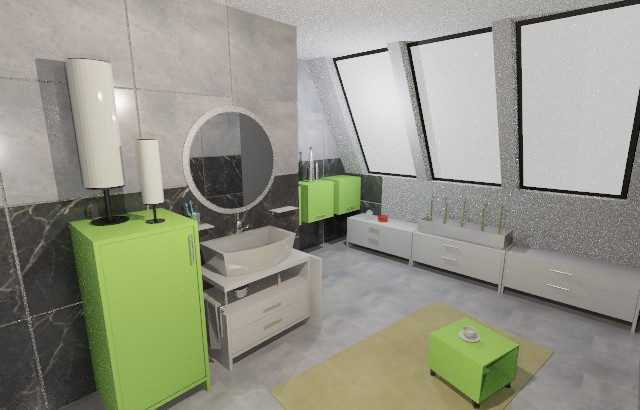
\includegraphics[width=\linewidth]{rough-reflections/small-off.png}
\end{minipage}\hfill
\begin{minipage}{.46\linewidth}\centering\small\sffamily 开启反射降噪\par\smallskip
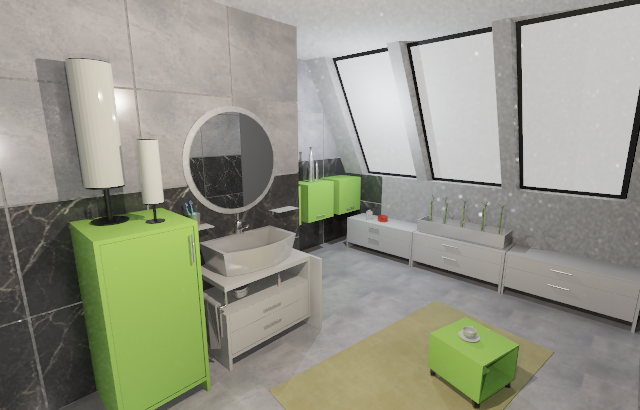
\includegraphics[width=\linewidth]{rough-reflections/small-on.png}
\end{minipage}\par\smallskip
\panelimage{.30\linewidth}{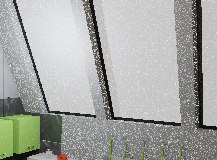
\includegraphics[width=\linewidth]{rough-reflections/detail-off.png}}{每像素一条光线}
\hfill\panelimage{.30\linewidth}{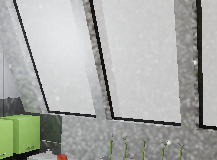
\includegraphics[width=\linewidth]{rough-reflections/detail-on.png}}{同一次采样，开启降噪}
\hfill\panelimage{.30\linewidth}{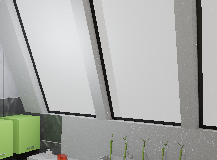
\includegraphics[width=\linewidth]{rough-reflections/detail-reference.png}}{每像素 256 次采样的平均值}
\caption{上排是 RTXGI Bathroom 在编辑器中的最终画面。下排单独查看 TAA 之前的窗框与墙面，三图使用相同的显示曲线。}
\end{figure}

固定相机与光照，对小画幅另取 256 组反射方向求平均，把它作为参照。把所有像素的线性红、绿、蓝三个分量分别和参照相减，平方后取平均，误差从 \roughRawMSE{} 降到 \roughFilteredMSE{}。将这 256 组分成两半，两张参照之间的同项误差为 \roughHalfMSE{}。

平均误差看不出哪条边变糊了。另一个测试让一面粗糙镜子照向亮灯牌，在镜子旁换上不同材质，每次都检查靠近分界处的两列像素。相邻材质换了颜色，或从金属换成非金属，这 192 个像素的结果都与旁边留空时相同。背景和理想镜面也分别比较了开关前后的颜色，每个像素都保持原值。浴室全图另查了每条反射光线是否命中物体，开启降噪后记录仍逐个相同。

\newpage
\section{反射追踪与降噪耗时}
两组渲染都使用浴室的原相机。第一组固定宽度为 640 像素，第二组按场景面板实际尺寸绘制。每种尺寸各抓两帧，只改「反射降噪」开关。RenderDoc 回放中，两帧追踪得到的原始反射逐字节相同，再比较它们各自花了多少时间。

{\smalltable\noindent\begin{tabularx}{\linewidth}{@{}Xlrrrr@{}}\toprule
画幅（像素）& 降噪 & 追踪（ms） & 降噪（ms） & 合计（ms） & 暂存（MiB）\\\midrule
\roughTimingRows
\bottomrule\end{tabularx}\par}

在 RTX 5070 Ti Laptop GPU 上捕获 Debug x64 编辑器，再用 RenderDoc 1.47 预热一次、回放 11 次。事件 556 负责追踪，开启时事件 568 执行降噪。「合计」先把同一次回放的耗时相加，再取中位数。两次捕获的追踪时间也有差异，所以最后两行的合计差值包含两部分。开关前后整帧都绘制 195 次，计算命令从 10 次增至 11 次。每个像素额外保存 16 字节的原始倒影，这块显存可以留给下一帧继续使用。

要判断打开浴室时该用哪个设置，我们还测了一整帧。关闭 RenderDoc 和 Vulkan 验证层，保留相同机位和面板原尺寸。三种设置轮换启动，各运行三次。每种设置记录 72 帧重新绘制的画面和 48 帧继续显示已有场景图的画面，从主线程开始处理这一帧一直计时到呈现返回，包含等待显卡的时间。

{\smalltable\noindent\begin{tabularx}{\linewidth}{@{}Xrrr@{}}\toprule
& \multicolumn{2}{c}{重新绘制（ms）}& 显示已有图（ms）\\
\cmidrule(lr){2-3}\cmidrule(l){4-4}
浴室的反射设置 & 中位数 & P95 & 中位数\\\midrule
\roughEditorRows
\bottomrule\end{tabularx}\par}

开启 SSR 的两行都允许射线离开屏幕后继续查询场景。重画时，这两行都比关闭 SSR 用时长。开启降噪的一组整帧中位数略低，但事件 568 本身占用了 0.350 毫秒。三轮启动测到的整帧用时也有起伏，暂不能用这组整帧差值判断降噪让引擎加速。

截帧还记录了 CPU 调用 \code{vkQueueSubmit} 把命令交给显卡用了多久。关闭降噪时，提交追踪用 \roughSubmitOff{} 微秒。开启时，提交追踪用 \roughSubmitOn{} 微秒，再提交降噪用 \roughSubmitFilter{} 微秒。这三个读数均来自捕获的第 24 帧，各只有一次。随后的等待以及显卡执行命令的时间需要另外计量。

浴室因此默认关闭 SSR。在场景面板打开 SSR 即可看到带降噪的屏幕内外倒影。后续可在 Vulkan 后端将追踪和降噪记进同一次提交，标清追踪写完、降噪才可读取的顺序。复测时沿用本页的两组计时，看减少一次提交和等待能省下多少整帧时间。

\readings{\href{run:../profiling/rough-reflections/bathroom.json}{GPU 逐次计时与误差}\quad
\href{run:../profiling/rough-reflections/editor-timing.json}{编辑器逐帧耗时}\quad
\href{run:../profiling/rough-reflections/editor-submits.json}{CPU 提交记录}\quad
\refitem{https://www.uni-ulm.de/fileadmin/website_uni_ulm/iui.inst.100/institut/Papers/atrousGIfilter.pdf}{Dammertz 等，HPG 2010，§2.2}}
